\chapter{Resultados}\label{cap:resultados}

\section{Treinamento e custo computacional}

O treinamento foi concluído em três sessões, totalizando aproximadamente 30 h 58 min. O estado final registra 200.000 iterações, 199.916 atualizações efetivamente aplicadas pelo otimizador e 85 atualizações puladas pelo escalonador de AMP. Isso corresponde a aproximadamente 0,0425\% das tentativas de atualização. A diferença entre iterações e atualizações ocorre quando a precisão mista detecta valores numéricos inadequados e evita aplicar aquela atualização.

O pico de memória alocada pelo PyTorch foi de aproximadamente 5,58 GiB e o pico observado pela telemetria do dispositivo foi 7.417 MiB. A avaliação oficial levou 2.568,48 s (42,8 min) e a extração da malha levou 109,13 s (1,82 min). A Tabela~\ref{tab:custo} reúne esses valores.

\begin{table}[H]
\centering
\caption{Resumo da execução final.}
\label{tab:custo}
\begin{tabular}{lr}
\toprule
\textbf{Medida} & \textbf{Valor} \\
\midrule
Iteração final & 200.000 \\
Atualizações efetivas & 199.916 \\
Atualizações puladas por AMP & 85 \\
Tempo de treinamento & 30 h 58 min \\
Pico PyTorch & 5,58 GiB \\
Pico da telemetria & 7.417 MiB \\
Tempo de avaliação & 2.568,48 s \\
Tempo de meshing & 109,13 s \\
\bottomrule
\end{tabular}
\end{table}

A Tabela~\ref{tab:custo} mostra que o custo se concentra no treinamento por cena: avaliação e extração da malha somaram menos de 45 minutos, enquanto o treinamento consumiu quase 31 horas. Nesse regime, a cadeia prepara previamente um ambiente para simulação; ela não reconstrói a cena durante a execução de uma tarefa robótica.

\section{Síntese de vistas}

A Tabela~\ref{tab:metricas_neurais} reúne as médias do avaliador oficial sobre 100 vistas de teste. As três primeiras colunas medem a aparência das imagens: PSNR e SSIM aumentam com a semelhança à referência, enquanto LPIPS diminui quando a distância perceptual é menor. As seis colunas seguintes medem a correspondência das máscaras de instância em exigências crescentes de sobreposição. A média oficial coincide com a agregação dos resultados por vista. Os valores de imagem descrevem a projeção observada pelas câmeras, mas não medem a posição da superfície tridimensional.

\begin{table}[H]
\centering
\small
\caption{Métricas do avaliador oficial na cena \textit{study}.}
\label{tab:metricas_neurais}
\begin{tabular}{rrrrrrrrr}
\toprule
PSNR & SSIM & LPIPS & AP50 & AP75 & AP80 & AP85 & AP90 & AP95 \\
\midrule
41,1100 & 0,9875 & 0,0260 & 0,9956 & 0,9911 & 0,9849 & 0,9769 & 0,9311 & 0,7192 \\
\bottomrule
\end{tabular}
\end{table}

\subsection{Comparação com os resultados publicados do DM-NeRF}

A reprodução pode ser comparada diretamente aos valores publicados por \citet{wang2023dmnerf} para a mesma cena \textit{study} do DM-SR. Essa comparação é distinta de um novo baseline: seu objetivo é verificar se o estágio neural reproduz o comportamento reportado pelo método de origem antes de analisar as transformações propostas nesta dissertação. A Tabela~\ref{tab:repro_dmnerf} apresenta os valores.

\begin{table}[H]
\centering
\small
\caption{Comparação entre a reprodução desta dissertação e os resultados publicados para a cena \textit{study} do DM-SR.}
\label{tab:repro_dmnerf}
\begin{tabular}{lrrrr}
\toprule
\textbf{Fonte} & \textbf{PSNR (dB)} & \textbf{SSIM} & \textbf{LPIPS} & \textbf{AP$_{0,75}$ (\%)} \\
\midrule
Wang et al. (2023) & 41,08 & 0,987 & 0,026 & 98,86 \\
Esta reprodução & 41,110 & 0,9875 & 0,0260 & 99,11 \\
\bottomrule
\end{tabular}
\end{table}

As diferenças são de 0,03 dB em PSNR, 0,0005 em SSIM, aproximadamente zero em LPIPS na precisão reportada e 0,25 ponto percentual em AP$_{0,75}$. Como PSNR, SSIM e AP aumentam com a qualidade e LPIPS diminui, a proximidade ocorre em todas as direções esperadas das métricas. Com uma única cena, esses desvios não sustentam uma análise de significância estatística; eles mostram que a execução reproduz proximamente os valores publicados para \textit{study}.

O mesmo artigo reporta, para a cena \textit{study}, AP$_{0,75}$ de 96,86\% para Mask R-CNN e 97,88\% para Swin Transformer, ambos ajustados por cena, contra 98,86\% do DM-NeRF publicado. A reprodução desta dissertação obteve 99,11\%. Em relação aos valores publicados dos dois baselines 2D, a diferença é de 2,25 e 1,23 pontos percentuais, respectivamente. Esses números são usados como referência de literatura e não como reexecução independente dos baselines.

A Figura~\ref{fig:render_comparison} compara as vistas 0, 33, 66 e 99 com as renderizações correspondentes. Cada coluna deve ser lida verticalmente: a primeira linha é a referência, a segunda é a imagem gerada pelo DM-NeRF e a terceira marca a diferença absoluta. Como as duas primeiras linhas são visualmente próximas, a diferença foi ampliada por um fator cinco apenas para visualização. As áreas claras nessa terceira linha se concentram em contornos, sombras e detalhes do mobiliário, enquanto as superfícies maiores mantêm aparência semelhante.

\begin{figure}[H]
  \centering
  \begin{minipage}{0.88\textwidth}
    \centering
    \small (a) Referência DM-SR\par\vspace{0.25em}
    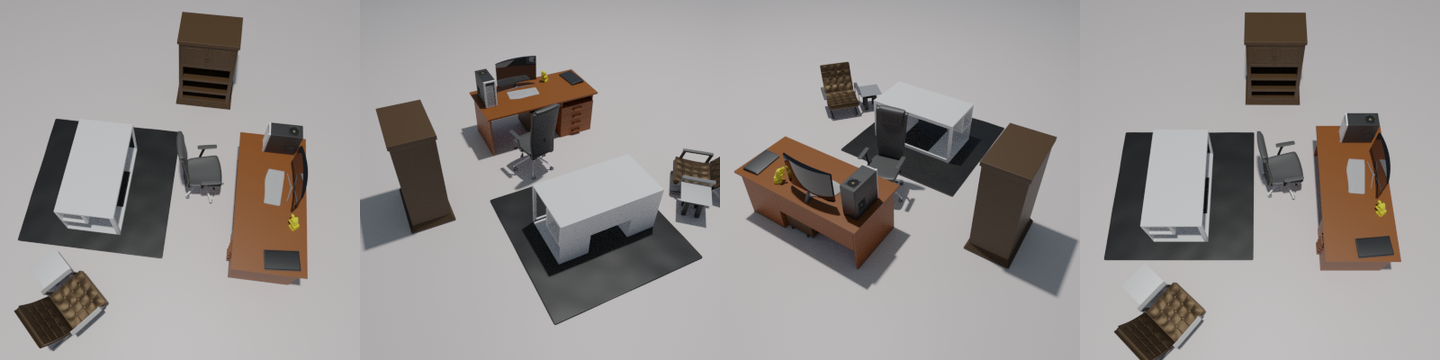
\includegraphics[width=\linewidth]{render_reference_row.png}\par\vspace{0.65em}
    \small (b) Renderização DM-NeRF\par\vspace{0.25em}
    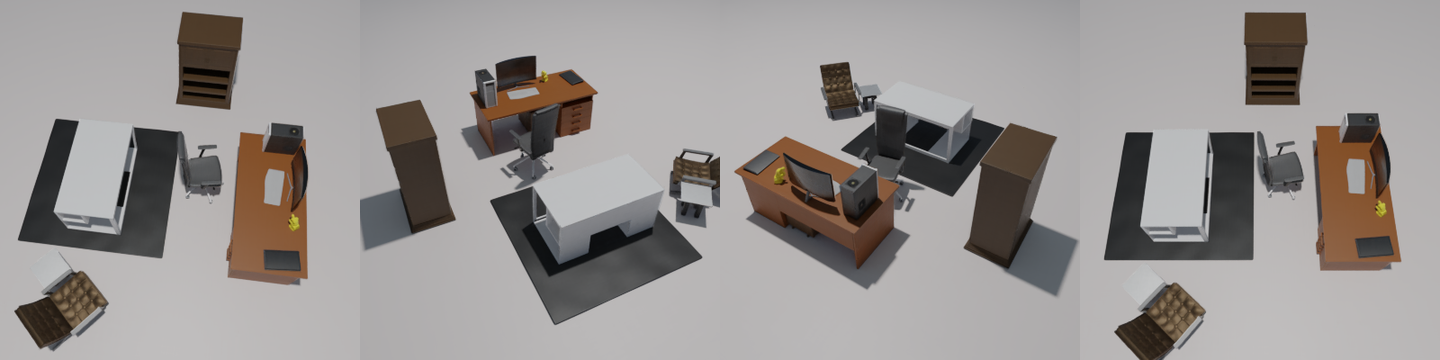
\includegraphics[width=\linewidth]{render_prediction_row.png}\par\vspace{0.65em}
    \small (c) Diferença absoluta ampliada $5\times$\par\vspace{0.25em}
    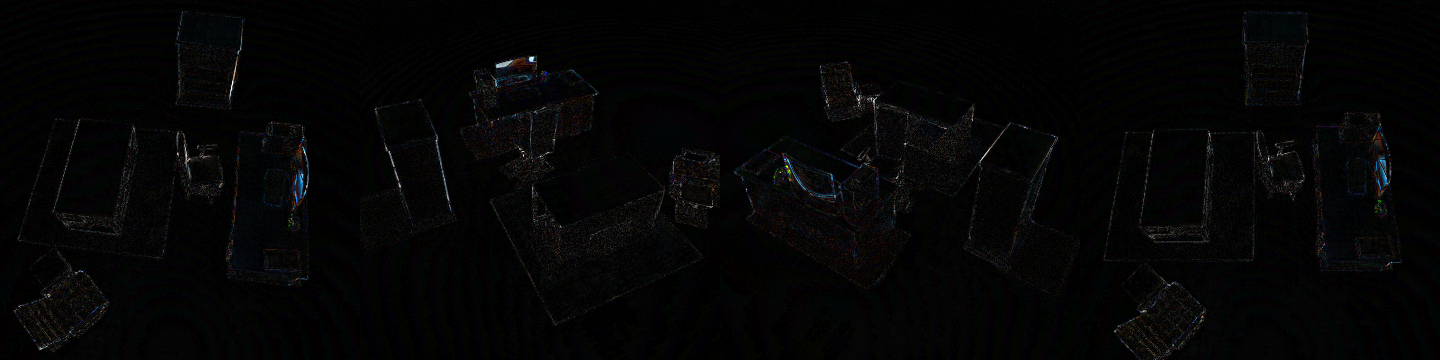
\includegraphics[width=\linewidth]{render_difference_row.png}
  \end{minipage}
  \caption{Síntese de vistas nas posições 0, 33, 66 e 99. A ampliação da diferença em (c) torna visíveis discrepâncias locais sem alterar as imagens comparadas.}
  \label{fig:render_comparison}
\end{figure}

\section{Decomposição de instâncias}

Os APs, para os quais valores maiores indicam melhor detecção e correspondência das máscaras, permanecem próximos de 1,0 nos limiares de IoU menos restritivos e diminuem quando a coincidência exigida se aproxima de 0,95. O AP50 é 0,9956, enquanto o AP95 é 0,7192. Esse comportamento indica que a correspondência geral das instâncias é mantida na maior parte das vistas, mas diferenças de contorno e pequenas regiões passam a afetar a métrica no limiar mais estrito. Como o protocolo fornece máscaras 2D durante o treinamento, os valores não demonstram descoberta de instâncias sem supervisão.

A Figura~\ref{fig:instancias_2d} compara os mapas de referência e predição nas mesmas quatro vistas. Cada cor identifica um objeto individual, e não sua categoria. A terceira linha marca em magenta os pixels cujo ID difere entre os dois mapas. O leitor deve observar que as regiões centrais dos objetos permanecem em grande parte iguais, enquanto as discordâncias se concentram nas fronteiras e em estruturas pequenas. Isso explica por que o AP permanece alto em IoU 0,50 e diminui quando a sobreposição exigida chega a 0,95.

\begin{figure}[H]
  \centering
  \begin{minipage}{0.88\textwidth}
    \centering
    \small (a) IDs de referência\par\vspace{0.25em}
    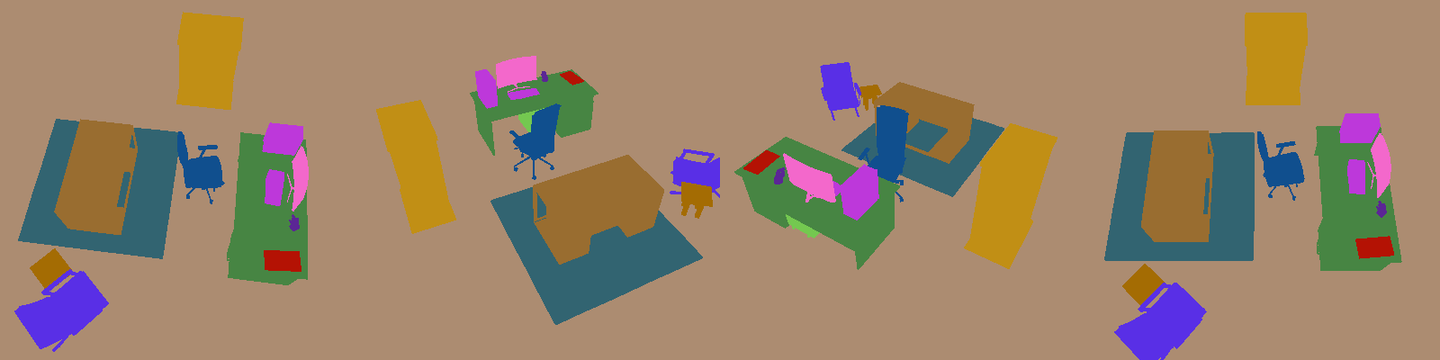
\includegraphics[width=\linewidth]{instance_reference_row.png}\par\vspace{0.65em}
    \small (b) IDs preditos pelo DM-NeRF\par\vspace{0.25em}
    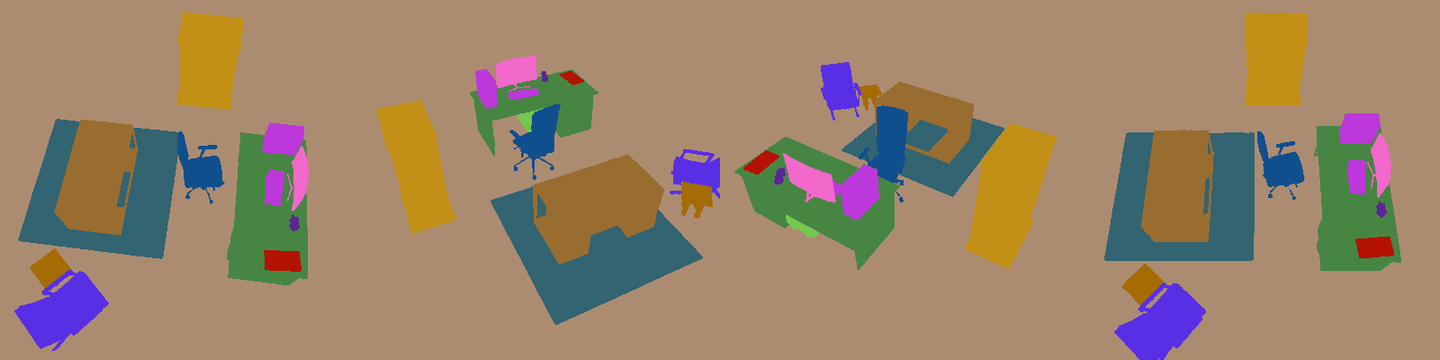
\includegraphics[width=\linewidth]{instance_prediction_row.png}\par\vspace{0.65em}
    \small (c) Pixels com IDs divergentes\par\vspace{0.25em}
    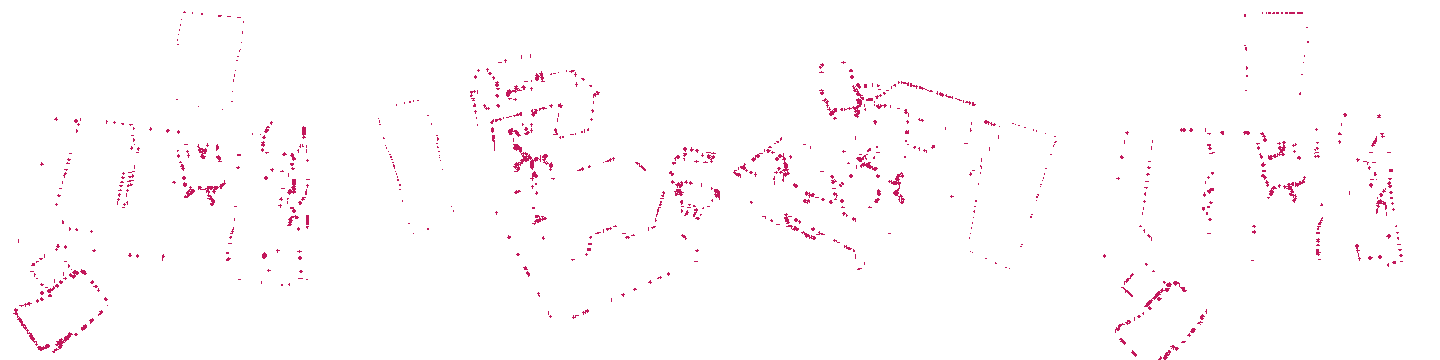
\includegraphics[width=\linewidth]{instance_difference_row.png}
  \end{minipage}
  \caption{Decomposição de instâncias nas vistas 0, 33, 66 e 99. Em (a) e (b), as cores identificam IDs, não classes semânticas; em (c), magenta indica divergência entre referência e predição.}
  \label{fig:instancias_2d}
\end{figure}

\section{Geometria extraída (A0)}

A malha A0 final contém 356.272 vértices e 710.928 faces. A comparação visual com a referência DM-SR e o COLMAP aparece na Figura~\ref{fig:geom_qual}, sem repetir o mesmo enquadramento em uma figura isolada. A estrutura global da sala e dos objetos principais é reconhecível, mas a visualização também mostra regiões ruidosas e superfícies que não formam volumes fechados.

A Tabela~\ref{tab:geom_dist} apresenta as distâncias médias e RMSE; em todas essas medidas, valores menores indicam maior proximidade entre as superfícies. As duas direções têm valores próximos: 4,34 cm da predição para a referência e 4,14 cm da referência para a predição. Essa proximidade entre as direções indica que o erro médio não é dominado apenas por pontos excedentes da reconstrução nem apenas por regiões ausentes da referência. Os RMSEs, maiores que as médias, mostram que alguns pontos estão mais afastados e recebem peso maior pelo erro quadrático.

\begin{table}[H]
\centering
\caption{Distâncias entre A0 e a referência DM-SR.}
\label{tab:geom_dist}
\begin{tabular}{lr}
\toprule
\textbf{Medida} & \textbf{Valor} \\
\midrule
Média predição $\rightarrow$ referência & 4,335 cm \\
Média referência $\rightarrow$ predição & 4,139 cm \\
Distância simétrica L1 & 8,474 cm \\
RMSE predição $\rightarrow$ referência & 5,757 cm \\
RMSE referência $\rightarrow$ predição & 4,940 cm \\
\bottomrule
\end{tabular}
\end{table}

Os resultados por limiar são apresentados na Tabela~\ref{tab:geom_threshold}. Precision mede a fração da reconstrução situada perto da referência; Completeness mede a fração da referência coberta pela reconstrução; e o F-score combina as duas medidas. Valores maiores são melhores. A 1 cm, somente cerca de 5\% dos pontos em cada direção encontram correspondência dentro do limiar. A 5 cm, Precision e Completeness passam de 0,75 e o F-score chega a 0,7750. Assim, a reconstrução representa melhor a estrutura quando se admite tolerância de 5 cm, sem sustentar coincidência fina em 1 cm.

\begin{table}[H]
\centering
\caption{Precision, Completeness e F-score da geometria A0.}
\label{tab:geom_threshold}
\begin{tabular}{rrrr}
\toprule
\textbf{Limiar} & \textbf{Precision} & \textbf{Completeness} & \textbf{F-score} \\
\midrule
1 cm & 0,04887 & 0,04724 & 0,04804 \\
2 cm & 0,20977 & 0,18398 & 0,19603 \\
5 cm & 0,79630 & 0,75478 & 0,77498 \\
\bottomrule
\end{tabular}
\end{table}

\section{Baseline geométrico externo: COLMAP}

O baseline COLMAP concluiu o PatchMatch e a fusão densa para as 300 vistas de treinamento, produzindo 5.800.316 pontos. Após a conversão para o sistema de coordenadas da malha e a restrição ao mesmo volume orientado empregado pelo meshing do DM-NeRF, 3.416.962 pontos permaneceram no suporte comum. A comparação usa uma amostra determinística de 200.000 pontos dessa nuvem, de modo a manter a mesma cardinalidade de A0 e da referência.

A Tabela~\ref{tab:colmap_geom} compara as duas reconstruções. A0 apresenta menor erro nas duas direções. A distância média da predição para a referência é 4,34 cm em A0 e 20,42 cm no COLMAP; no sentido referência para predição, os valores são 4,14 cm e 8,13 cm. A diferença entre as direções no COLMAP indica que parte relevante da superfície de referência possui pontos próximos, mas a nuvem contém espessamento e pontos afastados da superfície correta.

\begin{table}[H]
\centering
\small
\caption{Comparação geométrica entre A0 e o baseline COLMAP no mesmo suporte e com 200.000 pontos por conjunto.}
\label{tab:colmap_geom}
\begin{tabular}{lrr}
\toprule
\textbf{Medida} & \textbf{DM-NeRF A0} & \textbf{COLMAP} \\
\midrule
Média predição $\rightarrow$ referência & 4,335 cm & 20,418 cm \\
Média referência $\rightarrow$ predição & 4,139 cm & 8,129 cm \\
Distância simétrica L1 & 8,474 cm & 28,547 cm \\
RMSE predição $\rightarrow$ referência & 5,757 cm & 30,079 cm \\
RMSE referência $\rightarrow$ predição & 4,940 cm & 13,942 cm \\
\midrule
F-score a 1 cm & 0,0480 & 0,0285 \\
F-score a 2 cm & 0,1960 & 0,1288 \\
F-score a 5 cm & 0,7750 & 0,3721 \\
\bottomrule
\end{tabular}
\end{table}

A decomposição de Precision e Completeness ajuda a interpretar a diferença a 5 cm: A0 obtém 0,7963 e 0,7548, respectivamente, enquanto o COLMAP obtém 0,2710 e 0,5936. A completude do COLMAP é maior que sua precisão. Isso significa que sua nuvem chega perto de parte relevante da referência, mas uma parcela maior dos pontos reconstruídos permanece afastada da superfície correta. A Figura~\ref{fig:geom_qual} permite observar esse espessamento ao comparar as três colunas no mesmo enquadramento. A Figura~\ref{fig:geom_fscore} mostra, para ambos os métodos, o aumento do F-score quando a tolerância passa de 1 para 5 cm; barras maiores são melhores.

\begin{figure}[H]
  \centering
  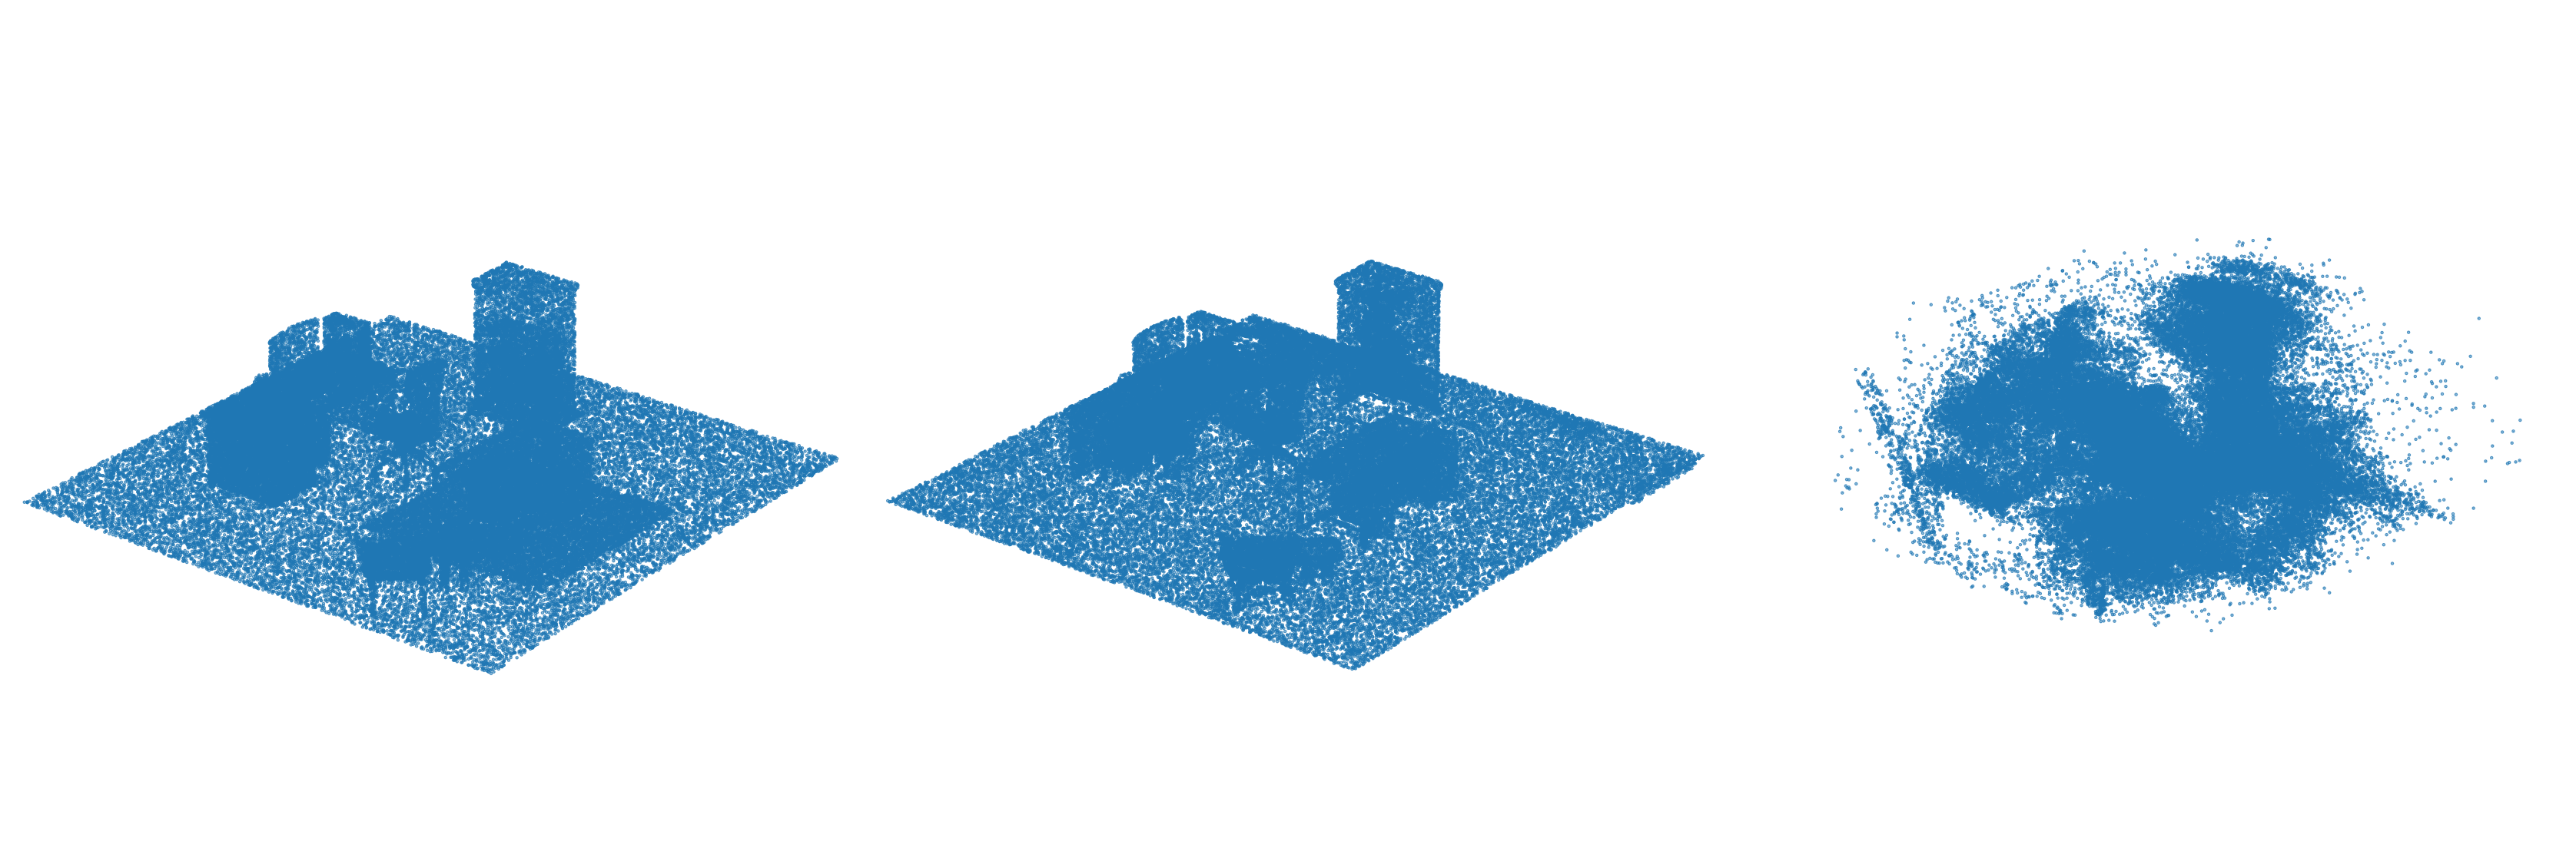
\includegraphics[width=\textwidth]{geometry_qualitative_comparison.png}
  \parbox{0.32\textwidth}{\centering\small (a) Referência DM-SR}\hfill
  \parbox{0.32\textwidth}{\centering\small (b) DM-NeRF A0}\hfill
  \parbox{0.32\textwidth}{\centering\small (c) COLMAP}
  \caption{Comparação qualitativa da geometria no mesmo sistema de coordenadas, suporte e enquadramento. A nuvem COLMAP apresenta maior dispersão e superfícies mais espessas.}
  \label{fig:geom_qual}
\end{figure}

\begin{figure}[H]
  \centering
  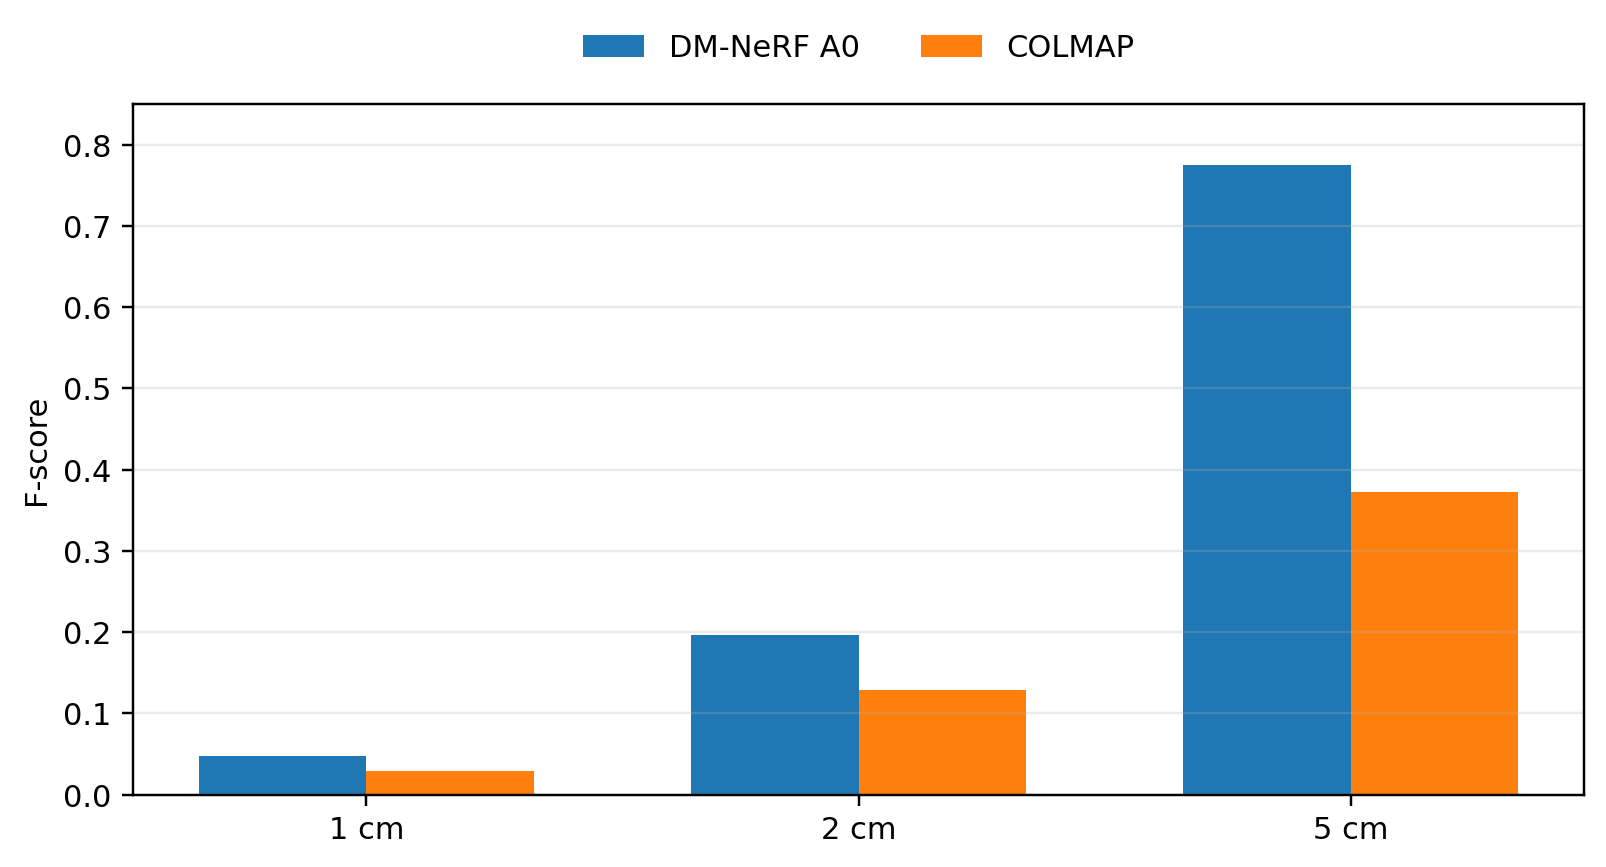
\includegraphics[width=0.82\textwidth]{geometry_fscore_comparison.png}
  \caption{F-score geométrico de A0 e COLMAP nos limiares de 1, 2 e 5 cm.}
  \label{fig:geom_fscore}
\end{figure}

\section{Separação estrutural (A1)}

A separação identificou 13 instâncias com faces homogêneas. Das 710.928 faces da malha original, 681.383 foram atribuídas a uma instância, enquanto 29.545 foram registradas como faces de fronteira. A Tabela~\ref{tab:a1} organiza essa contagem. A cobertura resultante é 95,844\%; nesse indicador, valores maiores representam maior preservação da topologia nas malhas individuais. A1 não melhora a geometria de A0: seu resultado é estrutural, pois transforma os IDs associados à malha em arquivos e modelos que podem ser manipulados separadamente. A cobertura não mede estanqueidade nem corrige erros geométricos da malha de origem.

\begin{table}[H]
\centering
\caption{Resumo da separação A1.}
\label{tab:a1}
\begin{tabular}{lr}
\toprule
Instâncias exportadas & 13 \\
Faces da malha A0 & 710.928 \\
Faces homogêneas exportadas & 681.383 \\
Faces de fronteira & 29.545 \\
Cobertura de faces homogêneas & 95,844\% \\
\bottomrule
\end{tabular}
\end{table}

A Figura~\ref{fig:a1} mostra a mesma reconstrução em dois pontos de vista. As mudanças de cor marcam as fronteiras entre IDs e permitem reconhecer quais partes se tornaram objetos distintos. A identidade empregada no processamento vem do vetor de IDs, não da cor armazenada em \texttt{mesh\_instances.ply}.

\begin{figure}[H]
  \centering
  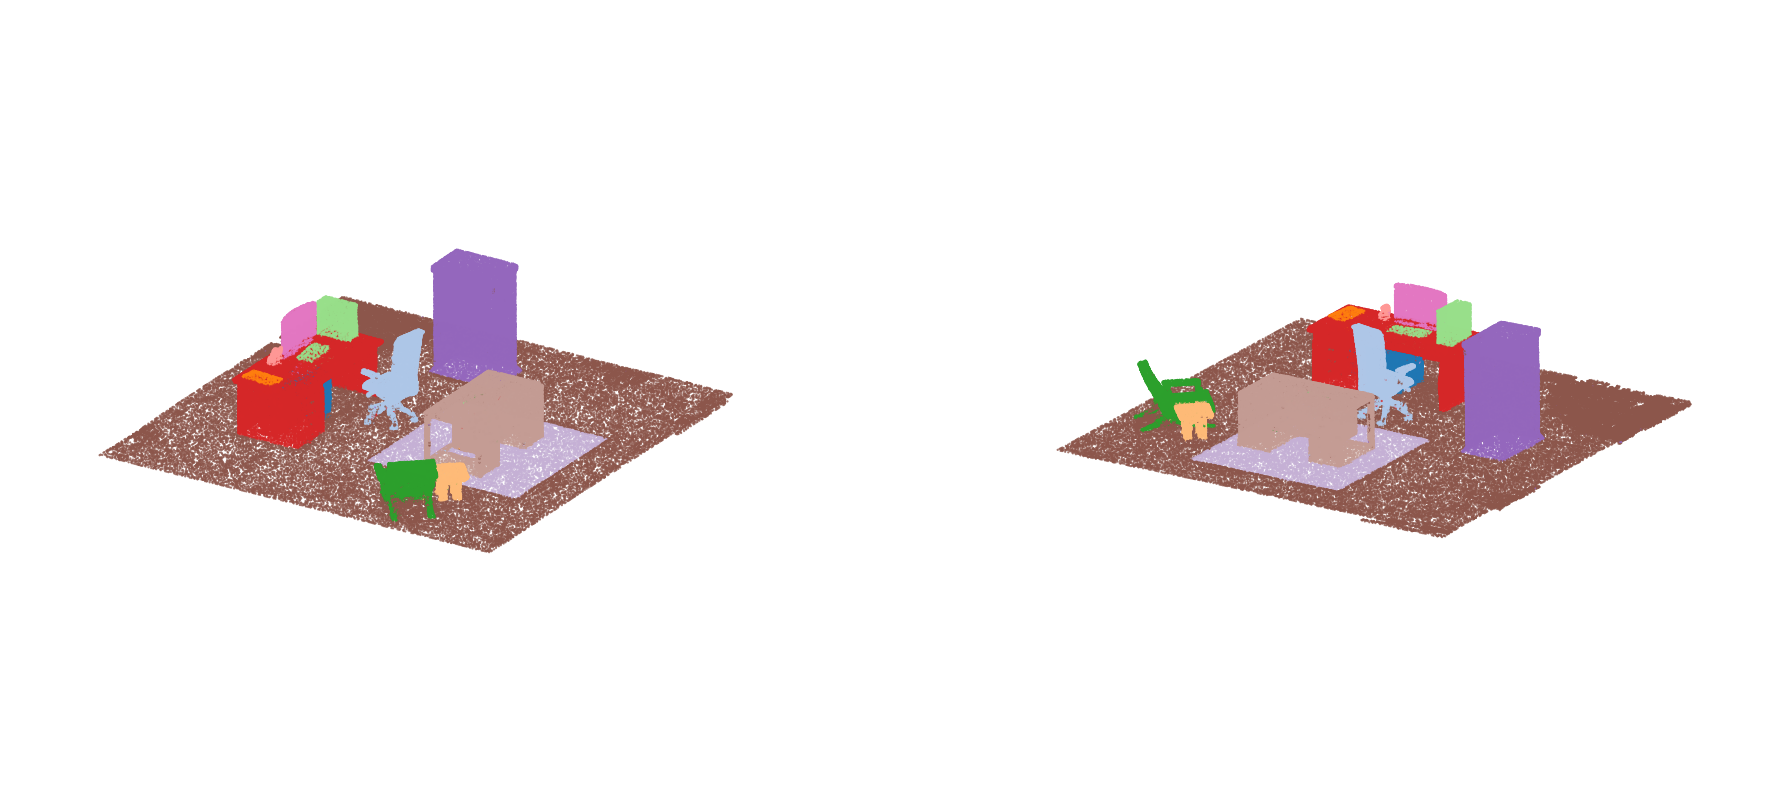
\includegraphics[width=\textwidth]{a1_instances.png}
  \caption{Visualização da reconstrução colorida por instância em dois pontos de vista. As cores são usadas somente para distinguir IDs.}
  \label{fig:a1}
\end{figure}

A individualização também foi verificada nos arquivos exportados por instância. Fragmentos e fronteiras permanecem visíveis em alguns objetos; por essa razão, a Figura~\ref{fig:a1} apresenta a cena completa colorida por ID, e a Figura~\ref{fig:gazebo_colorido} mostra posteriormente cada entidade carregada separadamente no Gazebo.

\section{Seleção e regularização do piso}

A heurística geométrica selecionou a instância 10. Ela foi a única instância a satisfazer simultaneamente os critérios de área, orientação, planaridade e altura. A instância 9 também apresenta grande fração horizontal e baixa altura, mas seu RMSE de 3,23 cm excede o limite de 3 cm definido antes da execução final. A seleção identifica um candidato geométrico e não constitui rótulo semântico de piso fornecido pelo DM-SR.

No RANSAC aplicado à instância selecionada, 77,11\% dos vértices ficaram a até 2 cm do plano estimado. Antes da projeção, a distância absoluta média era 2,051 cm, o RMSE era 5,722 cm e o P95 era 6,800 cm. O maior residual chegou a 1,64 m, indicando a presença de vértices associados ao mesmo ID afastados do plano principal. Esse valor não foi removido da análise.

A Tabela~\ref{tab:piso} compara o mesmo conjunto de vértices antes e depois da projeção. Para média absoluta, RMSE e P95, valores menores indicam maior proximidade ao plano; para a fração de inliers, valores maiores indicam que mais vértices estão a até 2 cm. A projeção de A2 leva os vértices selecionados ao plano, reduzindo média, RMSE e P95 a erro numérico. Essa redução ocorre por construção e descreve a planarização aplicada, não um aumento medido da fidelidade global da reconstrução. A consequência funcional é verificada separadamente pelo contato no Gazebo.

\begin{table}[H]
\centering
\caption{Métricas da instância 10 antes e depois da regularização.}
\label{tab:piso}
\begin{tabular}{lrr}
\toprule
\textbf{Medida} & \textbf{A1} & \textbf{A2} \\
\midrule
Média absoluta & 2,051 cm & $<10^{-12}$ cm \\
RMSE & 5,722 cm & $<10^{-12}$ cm \\
P95 & 6,800 cm & $<10^{-12}$ cm \\
Fração de inliers (2 cm) & 77,11\% & 100\% \\
\bottomrule
\end{tabular}
\end{table}

\begin{figure}[H]
  \centering
  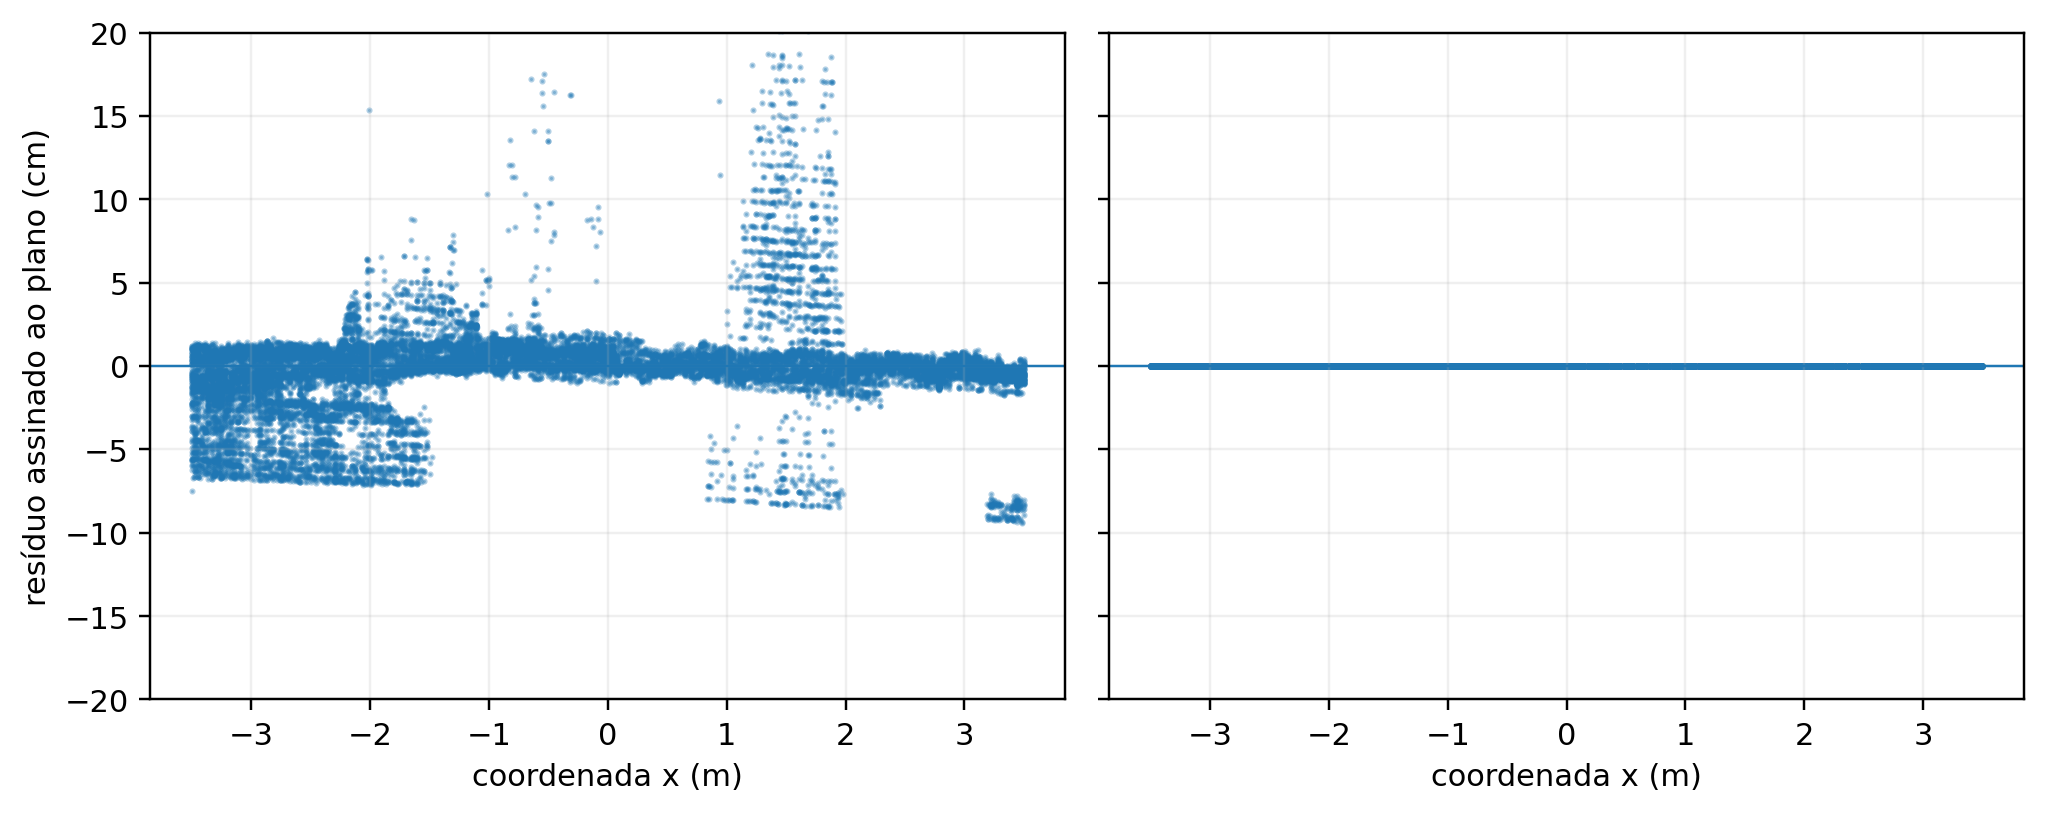
\includegraphics[width=\textwidth]{floor_residual_comparison.png}
  \caption{Resíduo assinado ao plano da instância 10 antes e depois da regularização. À esquerda, A1; à direita, A2. O eixo vertical é limitado a $\pm20$ cm para leitura da distribuição principal; o residual máximo de A1, 1,64 m, permanece reportado no texto e nas métricas.}
  \label{fig:piso}
\end{figure}

Na Figura~\ref{fig:piso}, a concentração dos pontos de A2 em torno de zero confirma o efeito da projeção. Em A1, a dispersão mostra as irregularidades do candidato original; o limite vertical de $\pm20$ cm permite ler a região principal sem ocultar do texto o residual máximo de 1,64 m.

\section{Integração no Gazebo Classic}

A Tabela~\ref{tab:gates} deve ser lida como uma sequência de propriedades distintas. G0 verifica a estrutura dos arquivos; G1 verifica se o Gazebo carrega os mundos; G2 verifica se um objeto separado pode ser deslocado sem mover os demais; e G3 verifica o contato em um ponto da superfície regularizada. A validação G0 passou para as três condições. A0 gerou um modelo correspondente à malha completa; A1 e A2 geraram 13 modelos independentes, com caminhos relativos para os arquivos de malha e correspondência entre os elementos visuais e de colisão.

Os testes de execução foram realizados no Gazebo Classic 11.10.2. Em G1, os mundos A0, A1 e A2 foram carregados e permaneceram ativos durante a janela de verificação. Foram observados apenas avisos relativos à aparência visual padrão, sem erros de carregamento das geometrias usadas nos testes.

Em G2, a instância \texttt{instance\_006} da condição A1 foi deslocada em 0,25 m no eixo $x$ por meio da interface do Gazebo. A pose consultada antes da operação era $(0,0,0)$ m e, após o comando, a coordenada $x$ passou para 0,25 m. A operação foi dirigida somente a esse modelo, demonstrando que a separação de A1 foi materializada em entidades endereçáveis de forma independente no simulador.

O teste G3 utilizou uma caixa dinâmica de 10 cm de lado e massa de 0,2 kg, posicionada com centro em $z=0,65$ m sobre uma região do candidato a piso regularizado. A primeira pose foi registrada seis segundos após o início da simulação, já depois da queda. Nesse instante, o centro da caixa estava em $z=0,093811$ m; oito segundos depois, estava em $z=0,093806$ m, variação de aproximadamente 5 $\mu$m.

Considerando metade da altura da caixa, sua face inferior permaneceu em $z=0,043806$ m. A altura calculada do plano regularizado no ponto $(x,y)=(3,07411,-3,31338)$ m, após a rotação comum de +Y para +Z usada na exportação, é $z=0,043810$ m. A diferença de aproximadamente 4 $\mu$m expressa a concordância numérica entre a pose registrada da face inferior da caixa e a altura calculada do plano no mesmo ponto, não uma medida de precisão física micrométrica do Gazebo. A caixa caiu aproximadamente 0,56 m, encontrou a superfície, não a atravessou no ponto ensaiado e permaneceu estável durante a segunda janela de observação; por esses critérios, G3 foi aprovado.

\begin{table}[H]
\centering
\caption{Resultado das verificações de integração com o Gazebo Classic.}
\label{tab:gates}
\begin{tabularx}{\textwidth}{>{\raggedright\arraybackslash}X c c c}
\toprule
\textbf{Verificação} & \textbf{A0} & \textbf{A1} & \textbf{A2} \\
\midrule
G0 -- validação estática & passou & passou & passou \\
G1 -- carregamento no Gazebo & passou & passou & passou \\
G2 -- manipulação independente & -- & passou & -- \\
G3 -- apoio/colisão do piso & -- & -- & passou \\
\bottomrule
\end{tabularx}
\end{table}

Para tornar a individualização visualmente verificável, a mesma cena A2 foi aberta com materiais de visualização distintos por instância. Essa alteração não modifica poses, geometrias de colisão nem os resultados G1--G3. Na Figura~\ref{fig:gazebo_colorido}, as cores diferentes mostram que os elementos foram carregados como modelos separados. A caixa vermelha no canto superior esquerdo corresponde ao corpo dinâmico usado no ensaio G3; sua presença permite localizar o teste pontual, mas a captura não mede por si só a qualidade do contato.

\begin{figure}[H]
  \centering
  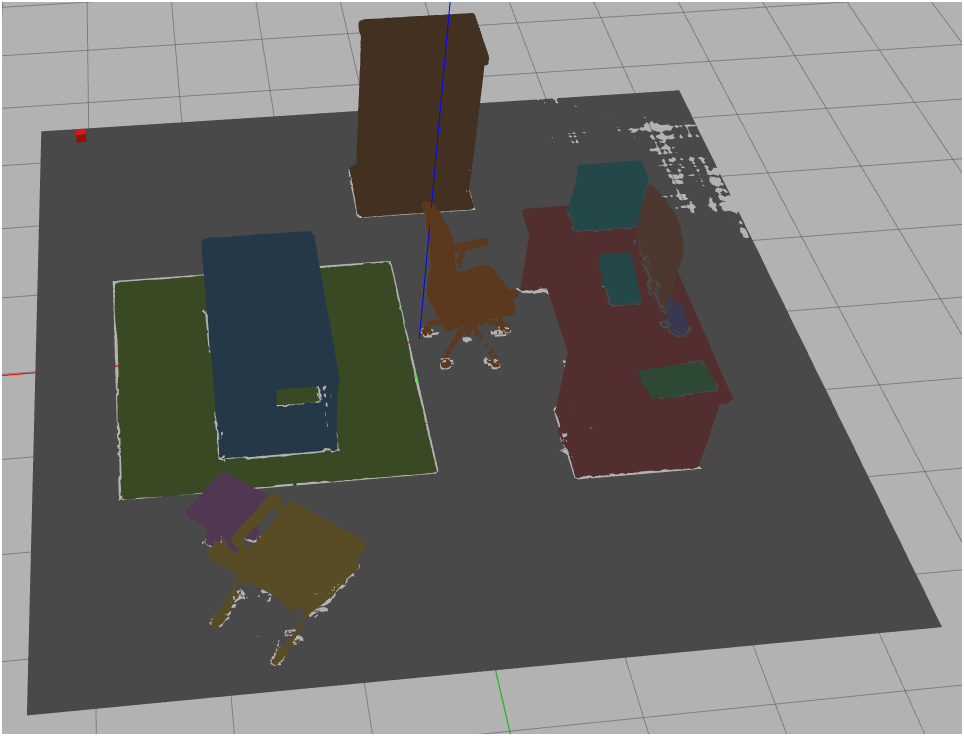
\includegraphics[width=0.88\textwidth]{gazebo_a2_colored.png}
  \caption{Cena A2 no Gazebo Classic com materiais visuais distintos por instância. As cores foram adicionadas somente para interpretação da figura; a geometria e as colisões são as mesmas usadas nos testes funcionais.}
  \label{fig:gazebo_colorido}
\end{figure}
